\documentclass{article}
\usepackage{listings}
\usepackage{graphicx}
\usepackage[slovene]{babel}
\usepackage{color}
\usepackage{amsmath}
\usepackage[usenames,dvipsnames]{xcolor}
\usepackage[hidelinks]{hyperref}
\usepackage{subcaption}
\usepackage{float}
\usepackage{rotating} 
\usepackage{hyperref}
\usepackage{caption}
\usepackage{siunitx}
\graphicspath{{./images/}}

\setlength{\parindent}{0pt}

\begin{document}

\title{Matematično-fizikalni praktikum \\[3mm] \large Naloga 10}
\author{Luka Papež}
\date{7.\ januar 2025}

\begin{center}
    
\includegraphics[width=8cm]{logo-fmf.png}
\end{center}

{
    \let\newpage\relax
    \maketitle
}

\maketitle
\newpage
\section{Naloga}
Spremljaj časovni razvoj začetnega stanja
\begin{equation*}
  \Psi(x,0)=\sqrt{\frac{\alpha}{\sqrt{\pi}}} e^{-\alpha^2 (x-\lambda)^2/2}
\end{equation*}
v harmonskem potencialu $V(x)=\frac12 kx^2$, kjer je v naravnih enotah $\alpha=k^{1/4}$, $\omega=\sqrt{k}$. 
Opazuj še razvoj gaussovskega valovnega paketa
\begin{equation*}
  \psi(x,0)=(2\pi \sigma_0^2)^{-1/4} e^{\ii k_0(x-\lambda)}e^{-(x-\lambda)^2/(2\sigma_0)^2}
\end{equation*}
v prostoru brez potenciala. 
V vseh obravnavanih primerih ugotovi in uporabi dovolj natančno metodo višjega reda.

\section{Uvod}
Enorazsežna nestacionarna Sch\"odingerjeva enačba
\begin{equation*}
  \left(i\hbar\Pd{}{t}-H\right)\psi(x,t)=0
\end{equation*}
je osnovno orodje za nerelativistični opis časovnega razvoja kvantnih stanj v različnih potencialih. Tu obravnavamo samo od časa neodvisne hamiltonske operatorje
\begin{equation*}
  H=-\frac{\hbar^2}{2m}\Pd[2]{}{x}+V(x)\>.
\end{equation*}
Z menjavo spremenljivk $H/\hbar\mapsto H$, $x\sqrt{m/\hbar}\mapsto x$ in $V(x\sqrt{m/\hbar})/\hbar\mapsto V(x)$, efektivno postavimo $\hbar=m=1$,
\begin{equation}
  H=-\frac12\Pd[2]{}{x}+V(x)\>.
  \label{eq:hamilton}
\end{equation}


Razvoj stanja $\psi(x,t)$ v stanje $\psi(x,t+\Delta t)$ opišemo s približkom
\begin{equation}
  \psi(x,t+\Delta t)=e^{-\ii H \Delta t} \psi(x,t)\approx \frac{1-\thalf \ii H \Delta t}{1+\thalf \ii H \Delta t}\psi(x,t)\>,
  \label{eq:razvoj}
\end{equation}
ki je unitaren in je reda $\mathcal{O}(\Delta t^3)$. Območje $a\leq x\leq b$ diskretiziramo na krajevno mrežo $x_j=a+j\Delta x$ pri $0\leq j<N$, $\Delta x = (b-a)/(N-1)$, časovni razvoj pa spremljamo ob časih $t_n=n\Delta t$. Vrednosti valovne funkcije in potenciala v mrežnih točkah ob času $t_n$ označimo $\psi(x_j,t_n)=\psi_j^n$ oziroma $V(x_j)=V_j$. Krajevni odvod izrazimo z diferenco
\begin{equation*}
  \Psi''(x)\approx \frac{\psi(x+\Delta x,t)-2\psi(x,t)+\psi(x-\Delta x,t)}{\Delta x^2}=\frac{\psi_{j+1}^n - 2\psi_j^n+\psi_{j-1}^n}{\Delta x^2}\>.
\end{equation*}
Ko te približke vstavimo v enačbo (\ref{eq:razvoj}) in razpišemo Hamiltonov operator po enačbi (\ref{eq:hamilton}), dobimo sistem enačb
\begin{equation*}
  \psi_j^{n+1}-\ii\frac{\Delta t}{4\Delta x^2}\left[\psi_{j+1}^{n+1}-2\psi_j^{n+1}+\psi_{j-1}^{n+1}\right] + \ii\frac{\Delta t}{2}V_j \psi_j^{n+1}=  \psi_j^{n}+\ii\frac{\Delta t}{4\Delta x^2}\left[\psi_{j+1}^{n}-2\psi_j^{n}+\psi_{j-1}^{n}\right] - \ii\frac{\Delta t}{2}V_j \psi_j^{n}\>,
\end{equation*}
v notranjih točkah mreže, medtem ko na robu ($j\leq 0$ in $j\geq N$) postavimo $\psi_j^n=0$. Vrednosti valovne funkcije v točkah $x_j$ uredimo v vektor
\begin{equation*}
\boldsymbol{\Psi}^n=(\psi_1^n,\ldots,\psi_{N-1}^n)^T
\end{equation*}
in sistem prepišemo v matrično obliko
\begin{equation*}
  \mathsf{A}\boldsymbol{\Psi}^{n+1}=\mathsf{A}^\ast \boldsymbol{\Psi}^n,\qquad
  \mathsf{A}=\begin{pmatrix}
  d_1 & a \\
  a   & d_2 & a \\
  & a & d_3 & a \\
  & & \ddots & \ddots & \ddots \\
  & & & a & d_{N-2} & a \\
  & & & & a & d_{N-1}
  \end{pmatrix}\>,
\end{equation*}
kjer je
\begin{equation*}
  b=\ii \frac{\Delta t}{2 \Delta x^2},\qquad a=-\frac{b}{2},\qquad d_j = 1+b+\ii \frac{\Delta t}{2}V_j\>.
\end{equation*}
Dobili smo torej matrični sistem, ki ga moramo rešiti v vsakem časovnem koraku, da iz stanja $\boldsymbol{\Psi}^n$ dobimo stanje $\boldsymbol{\Psi}^{n+1}$. Matrika $\mathsf{A}$ in vektor $\boldsymbol{\Psi}$ imata kompleksne elemente, zato račun najlažje opraviš v kompleksni aritmetiki
\newpage
\section{Rešitev}
\subsection{Harmonski potencial}
Reševanje začnemo z reševanjem časovnega razvoja začetnega stanja podanega v nalogi v harmonskem potencialu. Poglejmo si kako izgleda analitična rešitev. 
\begin{equation*}
  \psi(x,t)=\sqrt{\frac{\alpha}{\sqrt{\pi}}} \exp\left[-\frac12 \left(\xi-\xi_\lambda \cos\omega t\right)^2 - \ii \left(\frac{\omega t}{2}+\xi\xi_\lambda \sin\omega t - \frac14 \xi_\lambda^2 \sin 2 \omega t\right)\right]\>,
\end{equation*}
kjer je $\xi=\alpha x$, $\xi_\lambda=\alpha \lambda$. Parametre postavimo na $\omega=0.2$(oziroma $k=0.04$), $\lambda=10$. 
\begin{figure}[H]
	\centering
	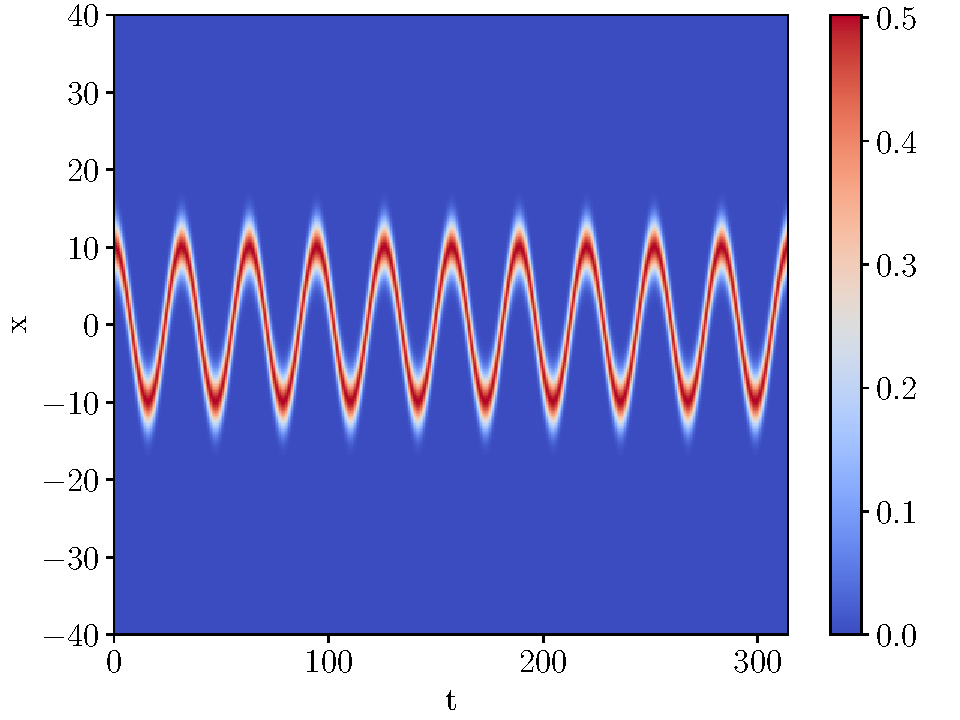
\includegraphics[width=0.7\linewidth]{anal.pdf}
	\caption{Analitični časovni razvoj podane začetne valovne funkcije za 10 oscilacij}
\end{figure}
Naša začetna valovna funkcija v razvoju skozi čas oscilira, kar je pričakovano za harmonični potencial. Zdaj smo pridobili podatek kakšna je oblika naše rešitve in začnemo z numeričnim reševanjem. V uvodu je natančno opisan pristop, kjer drugi odvod aproksimiramo z dvema členoma in je napaka $\mathscr{O}(h^2)$, kjer je $h$ velikost koraka. Ta približek lahko še izboljšamo z aproksimacijo z večimi členi.
\begin{equation}
y''(x) = \frac{1}{h^2} \sum_{k=-r}^r c_k^{(r)} y(x + kh) + O(h^{2r})
\end{equation}
Člene $c_k$ pa pridobimo iz podane tabele, ki je bolj natančno opisana v članku van Dijka.
\begin{figure}[H]
	\centering
	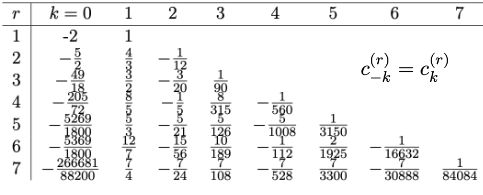
\includegraphics[width=0.7\linewidth]{table.png}
\end{figure}
Z metodo ostrega pogleda opazimo, da se tudi pri višjih členih simetričnost matrike sistema ohranja. S tem si precej olajšamo konstrukcijo, saj izven diagonalne člene potem le množimo s pripadajočim koeficientom. Vizualno so numerični rezultati precej nezanimivi, zato si poglejmo odstopanje od analitične rešitve za $r=1$ in $r=2$.
\begin{figure}[H]
    \centering
    \begin{subfigure}{0.45\textwidth}
        \centering
        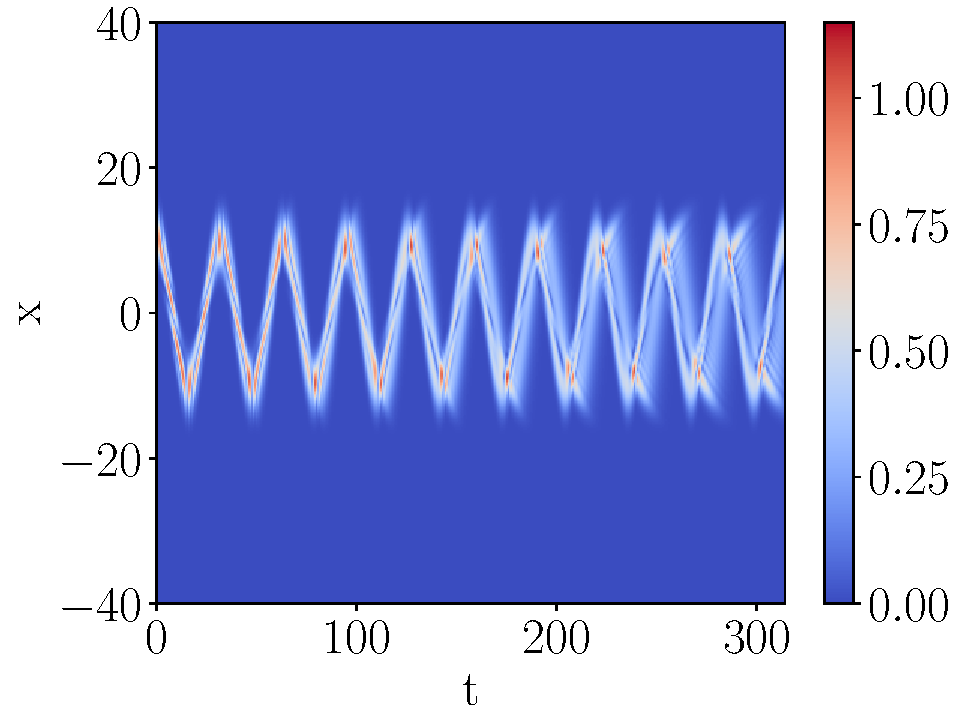
\includegraphics[width=\linewidth]{red1.pdf}
        \caption{$r=1$}
    \end{subfigure}
    \hfill
    \begin{subfigure}{0.45\textwidth}
        \centering
        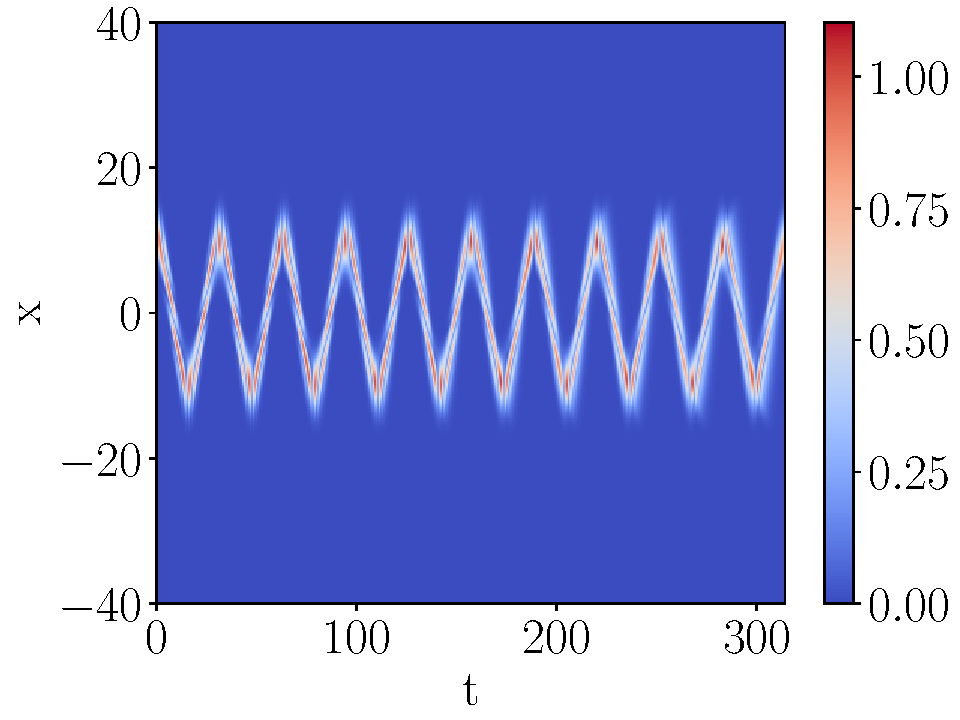
\includegraphics[width=\linewidth]{red2.pdf}
        \caption{$r=2$}
    \end{subfigure}
	\caption{Odstopanje numerične rešitve časovnega razvoja v harmoničnem potencialu od analitične rešitve}
\end{figure}
Oba reda sta na prvih desetih oscilacijah stabilna in imata približno enako obliko. Opazimo pa, da je $r=2$ precej bolj oster in nima vedno večjih čitnih odstopanj, kot jim ima $r=1$. Kljub izboljšanju in stabilnosti so napake precej velike zato si poglejmo še kako se redi spreminjajo med seboj.
\begin{figure}[H]
    \centering
    \begin{subfigure}{0.45\textwidth}
        \centering
        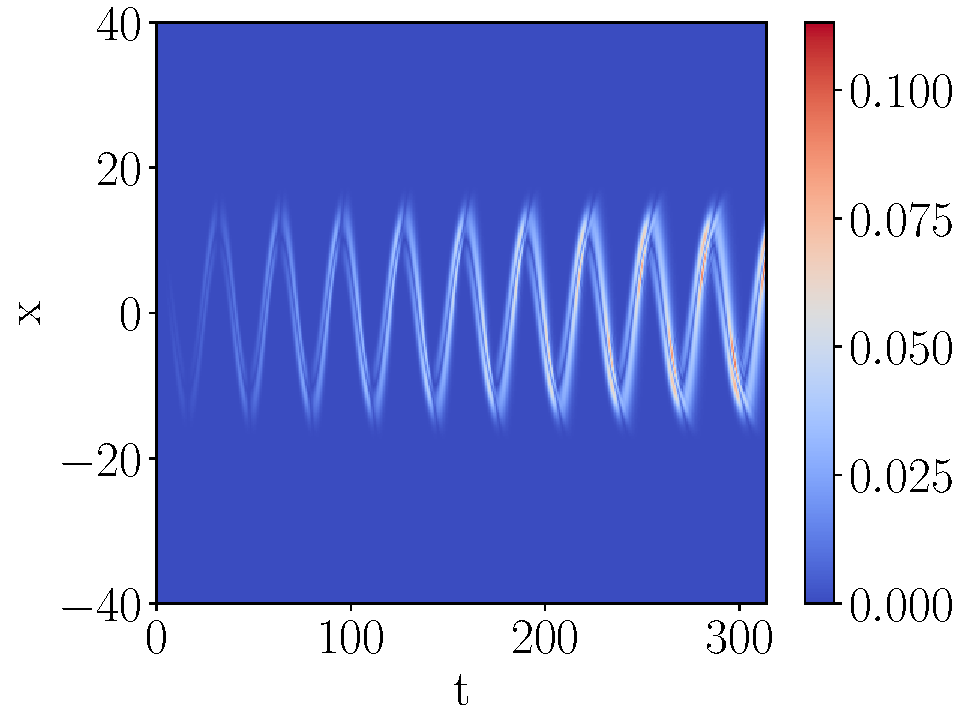
\includegraphics[width=\linewidth]{red27.pdf}
        \caption{Med $r=2$ in $r=7$}
    \end{subfigure}
    \hfill
    \begin{subfigure}{0.45\textwidth}
        \centering
        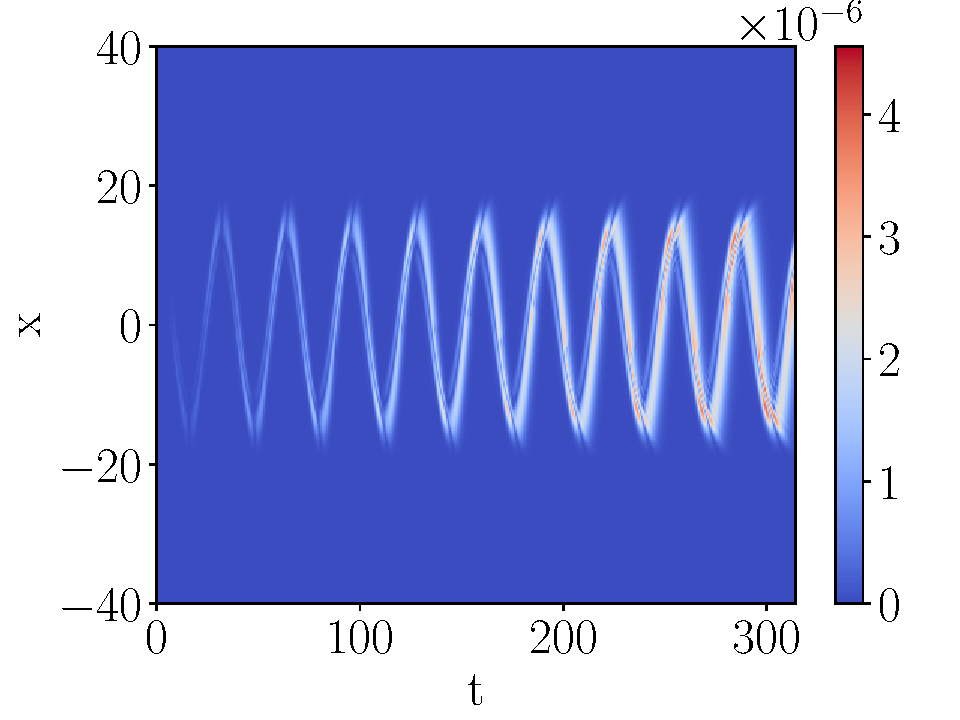
\includegraphics[width=\linewidth]{red67.pdf}
        \caption{Med $r=6$ in $r=7$}
    \end{subfigure}
	\caption{Odstopanje numeričnih rešitve časovnega razvoja v harmoničnem potencialu med različnimi redi}
\end{figure}
V primerjavi med $r=2$ in $r=7$ je precej očitno, da je metoda $r=2$ pri majhnih časih precej dobra a se sčasoma degradira. A odstopanje med metodama bistveno ne pripomore k natančnosti rešitve. Seveda zato pomislimo, da bi nadaljevali še z višjimi redi, a v primerjavi med redoma $r=6$ in $r=7$ jasno vidimo, da je sprememba reda $10^{-6}$. Kar je pričakovano glede na velikost koraka in tako vidimo, da je nadaljevanje nesmiselno. Kot še dodatna izboljšavo bi si lahko ogledali še višje rede Pad\'ejevega približka, ki ga uporabimo za približek eksponente funkcije.
\newpage
\subsection{Gaussov valovni paket}
Podobno kot v prejšnjem podpoglavju opazujemo časovni razvoj gaussovega valovnega paketa, ki se tokrat giblje prosto(brez potenciala).
Za vrednosti parametrov izberemo $\sigma_0=1/20$, $k_0=50\pi$, $\lambda=0.25$ in območje $[a,b]=[-0.5,1.5]$ ter $\Delta t=2\Delta x^2$. Analitična rešitev pa je
\begin{equation*}
  \psi(x,t)=\frac{(2\pi \sigma_0^2)^{-1/4}}{\sqrt{1+\ii t/(2\sigma_0^2)}} \exp\left[
    \frac{-(x-\lambda)^2/(2\sigma_0)^2+\ii k_0(x-\lambda)-\ii k_0^2 t/2}{1+\ii t/(2\sigma_0^2)}
    \right]
\end{equation*}
\begin{figure}[H]
	\centering
	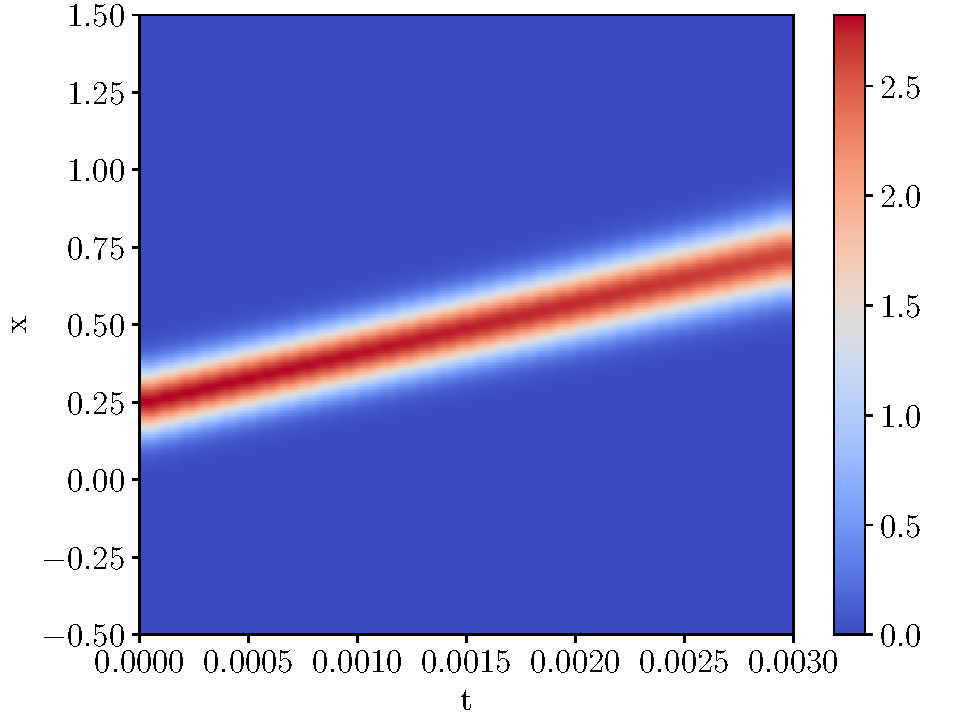
\includegraphics[width=0.7\linewidth]{analgauss.pdf}
	\caption{Analitični časovni razvoj Gaussovega valovnega paketa brez potenciala}
\end{figure}
V analitični rešitvi se Gaussov paket enakomerno premika naprej. Seveda nas precej bolj zanima kako se obnašajo naše numerične rešitve. Še enkrat si poglejmo odstopanja od analitične rešitve.
\begin{figure}[H]
    \centering
    \begin{subfigure}{0.45\textwidth}
        \centering
        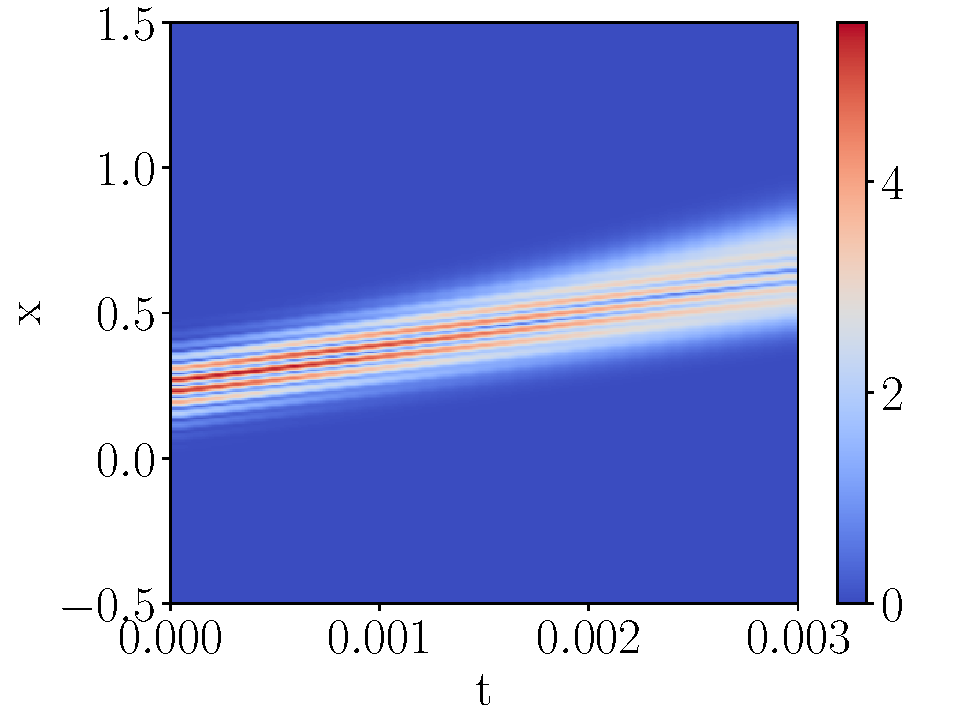
\includegraphics[width=\linewidth]{diff1.pdf}
		\caption{Odstopanje numerične rešitve $r=1$ časovnega razvoja Gaussovega paketa od analitične rešitve}
    \end{subfigure}
    \hfill
    \begin{subfigure}{0.45\textwidth}
        \centering
        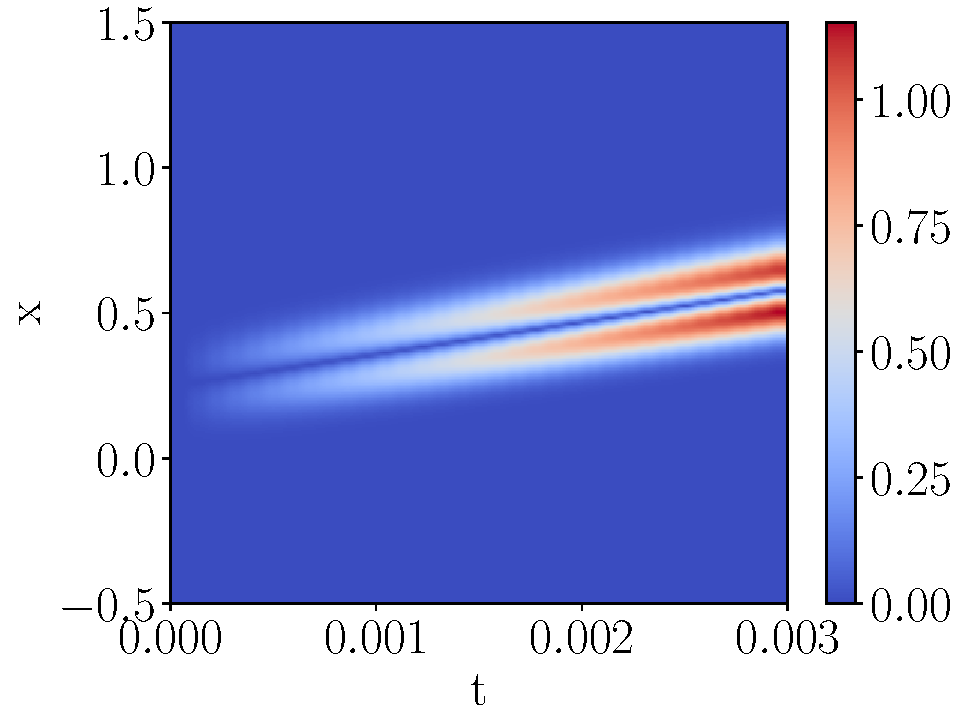
\includegraphics[width=\linewidth]{diff7.pdf}
        \caption{Odstopanje numeričnih rešitev časovnega razvoja Gaussovega paketa $r=1$ in $r=7$}
    \end{subfigure}
\end{figure}
Nova grafa nam potrdita ugotovitve iz razvoja v potencialu, kjer smo ugotovili, da so napake numeričnih rešitev precej velike in odstopanj tudi uporaba višjih redov bistveno ne izboljša. V primeru Gaussovega paketa je nestabilna rešitev precej vizualno zanimiva zato jo tudi podajam za konec kot zanimivost. Če bi bilo potrebno pa bi seveda tu lahko uporabljali bolj stabilne metode kot Crandall ali Numerov.
\begin{figure}[H]
	\centering
	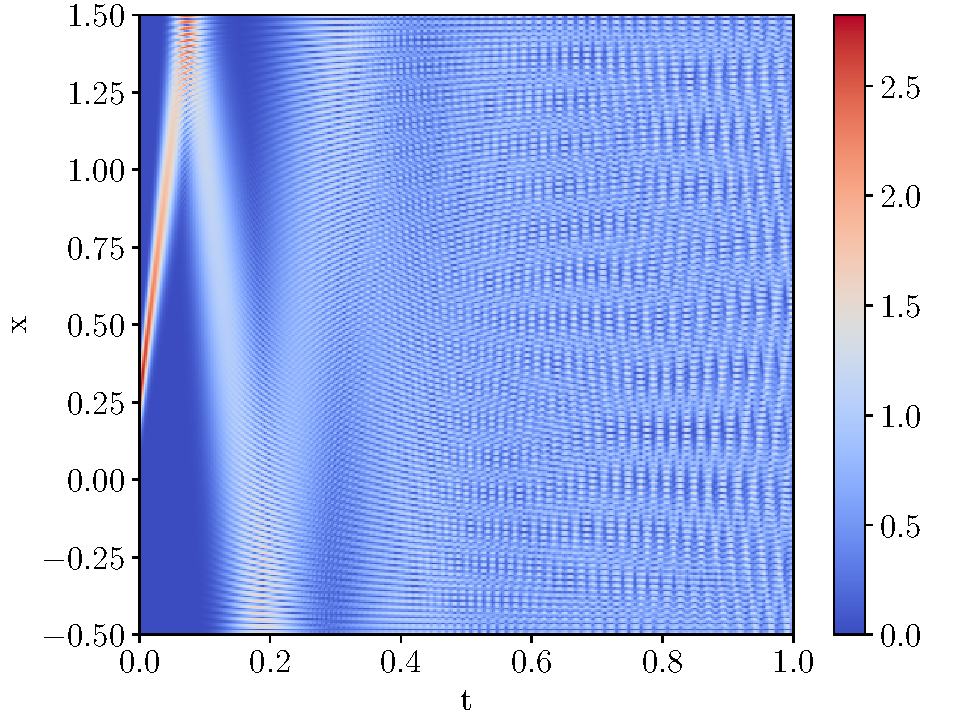
\includegraphics[width=0.7\linewidth]{nonstable.pdf}
	\caption{Primer nestabilne numerične rešitve razvoja Gaussovega paketa}
\end{figure}
\section{Zaključek}
V tej nalogi smo se ponovno srečali z reševanjem parcialnih diferencialnih s kompleksnimi števili. Tokrat so se metode izkazale za precej nenatančne, kar precej izstopa v primerjavi z dosedanjimi nalogami. Ponovno sem se tudi poskusil poigrati z uporabu grafične kartice, saj je v nalogi zelo pomembno množenje matrik. Ponovno se je izkazalo, da je bila uporaba grafične kartice precej počasnejša. To mi tudi sporoča, da je morda le ne znam pravilno uporabljati in moram posvetiti nekaj več časa k pravilnemu pristopu uporabe.\\
Dodajam še nekaj statistike o $1000$ naročenih pingvinih. Namesto $1000$ sem jih prejel $1038$ v sledečih paketih
\begin{table}[H]
\centering
\begin{tabular}{|c|c|}
\hline
	$N$ pingvinov v paketu & $N$ paketov \\ \hline
	50 & 1 \\ \hline
	51 & 1 \\ \hline
	52 & 3 \\ \hline
	53 & 7 \\ \hline
	102 & 2 \\ \hline
	103 & 2 \\ \hline
\end{tabular}
\end{table}
Od tega jih je bilo $100$ popraskanih $6$ neenakomernih in $2$ z barvnimi napakami. Poleg tega pa še $6$ takih, ki so imeli več kot eno napako. Tako je zaznanih $114$ pingvinov z napako, kar predstavlja $11\%$ oziroma, če upoštevamo presežek pingvinov $8\%$.
\end{document}
